\documentclass[twocolumn]{svjour3}
\usepackage{color}
\usepackage{soul}
\usepackage{cite}
\usepackage{array}
\usepackage{listings}
\usepackage{graphicx}
\usepackage{amsfonts}
\usepackage{amsmath, amsfonts, url, amssymb, graphics, algorithm2e,url} 
\usepackage{xspace}
%\usepackage{psnfss2e}
\usepackage{mathptmx}

\usepackage{url}
\newcommand{\starpar}[1]{\par{\footnotesize $\star$ \hl{#1}\par}}
\newcommand{\F}{{\mathbb F}}
\newcommand{\Z}{{\mathbb Z}}

\hyphenation{ec-dsa ec-dlp cu-rve}

\newcommand{\fl}{\textsc{Flu\-sh+\allowbreak Re\-load}\xspace}
\newcommand{\prpr}{\textsc{Prime+\allowbreak Probe}\xspace}

\newcommand{\myupcase}[1]{\uppercase{#1}}
%\newcommand{\myupcase}[1]{\textsc{#1}}

\lstset{basicstyle=\scriptsize,breaklines=true,breakindent=60pt,xleftmargin=20pt,numberstyle=\tiny,numbersep=5pt,language=C}

\begin{document}

\title{Recovering OpenSSL ECDSA Nonces Using the \fl Cache Side-channel Attack}
\author{Yuval Yarom \and Naomi Benger}
\institute{Yuval Yarom \and Naomi Benger \at The University of Adelaide, \email{yval@cs.adelaide.edu.au, naomi.benger@adelaide.edu.au}}

\maketitle

\begin{abstract}
We illustrate a vulnerability introduced to elliptic curve cryptographic protocols when implemented using a function of the OpenSSL cryptographic library.
For the given implementation using an elliptic curve $E$ over a binary field with a point $G\in E$, our attack can recover the majority of the bits of a scalar $k$ when $kG$ is computed using the OpenSSL implementation of the Montgomery ladder. 
For the Elliptic Curve Digital Signature Algorithm (\myupcase{ecdsa}) the scalar $k$ is intended to remain secret. 
Our attack recovers the scalar $k$ and thus the secret key of the signer and would therefore allow unlimited forgeries. 
This is possible from snooping on only one signing process and requires computation of less than one second on a quad core desktop when the scalar $k$ (and secret key) is around 571 bits.

\end{abstract}

\section{Introduction}
Elliptic curve cryptography (\myupcase{ecc})~\cite{miller85use,koblitz87elliptic} includes a number of public-key cryptographic protocols whose security relies on the computational intractability of the Elliptic Curve Discrete Logarithm Problem (\myupcase{ecdlp}): Given an elliptic curve over a finite field and two points~$G$ and~$H$ on the curve, find the scalar $k$ such that $H=kG$.

\myupcase{ecc} offers a higher encryption strength per key-bit than related methods whose security is reliant on the hardness of computing discrete logarithms in a finite field or factoring the product of large primes. Consequently, \myupcase{ecc} uses significantly shorter keys and offers faster operations than other methods, contributing to its rising popularity.

The Elliptic Curve Digital Signature Algorithm (\myupcase{ecdsa}) \cite{johnson01elliptic,fips,ansi962} is a standard
digital signature algorithm implemented using elliptic curves. One core operation of the \myupcase{ecdsa} algorithm, as in many \myupcase{ecc} protocols, is the scalar multiplication of a point on the elliptic curve by a pseudo-randomly generated secret nonce. The confidentiality of the nonce is paramount for the security of the algorithm. Past research indicates that partial exposure of nonce bits can be exploited for efficient attacks on the secret key~\cite{nguyen03insecurity,brumley11remote}.

OpenSSL~\cite{openssl} is a cryptographic software package that implements \myupcase{ecdsa}.
When using elliptic curves over a binary field $\mathbb{F}_{2^m}$, OpenSSL uses the 
Montgomery ladder~\cite{montgomery87speeding,joye03montgomery} algorithm to compute $kG$, the scalar multiplication of a publically known point $G$ by the secret nonce $k$.
One of the advantages of the Montgomery ladder is that it has a regular behaviour, performing
the same sequence of operations for each nonce bit, irrespective of the value of the bit.
This regular behaviour makes it more resilient to side-channel attacks~\cite{joye03montgomery,okeya00elliptic}.

While the operations performed by the algorithm are regular, their targets depend on the value of the bits of the nonce.
To apply the operations to the respective targets, the OpenSSL implementation uses a conditional branch based on the value of the bit. By tracing this branch an attacker can recover the values of the nonce bits and, consequently, break the cryptosystem. In this paper we present our use of the \fl cache side-channel attack~\cite{yarom13flush} to trace the branch in the OpenSSL implementation.

The \fl attack exploits a security weakness in the IA-32 and X86-64 architectures that allows processes
to monitor other processes read and execute access to shared memory pages.
Our spy program monitors access to both arms of the conditional branch and uses the information
collected from these probes to reconstruct the nonce. This attack is a threat to the security of any cryptographic protocol implemented using the OpenSSL scalar multiplication method when the scalar is intended to remain secret.

In this paper we illustrate the efficiency of the attack by analysing \myupcase{ecdsa} and recovering the secret key using only one signature at very little computational cost (in both time and memory). This attack is applicable when the malicious party has access to the memory of the targeted device.
This is  a reasonable assumption as could be the case when using, for example, a multi-user operating system, co-hosted virtual machines in a cloud computing environment or a computer victim to malware. 

The paper also presents new information on the limitation of the \fl attack.
We discuss spatial limitations, affecting the distance between multiple probes, and 
temporal limitations, affecting the probe resolution.
The results of this paper support the findings of Walter~\cite{walter04longer} that longer keys render a cryptographic algorithm more vulnerable to side-channel analysis.


The rest of this paper is organised as follows: in the following subsection we discuss related research. The next section presents background information on \myupcase{ecdsa}, the Montgomery ladder and the \fl attack. % and the validity of the assumption that an attacker has access to the computer's memory.
Section~\ref{sec:attack} describes our attack on the OpenSSL implementation of \myupcase{ecdsa}.
The results of the attack are analysed in Section~\ref{sec:results}.
We discuss the implications of the attack and suggest techniques for mitigation in Section~\ref{sec:discussion}.

\subsection{Related Work}\label{sec:related}
There have been a number of publications addressing the security issues of digital signatures when partial information is leaked~\cite{Howgrave-GrahamS01,gopalakrishnan07solving,nguyen03insecurity}. 

Gopalakrishnan et al.~\cite{gopalakrishnan07solving} presents algorithms for solving the \myupcase{ecdlp} using the additional information of some consecutive bits of the private key. These algorithms outperform the currently best known methods of solving the \myupcase{ecdlp} without the extra information or using exhaustive search on the remaining key space. In this work we do not focus on the \myupcase{ecdlp}.
Instead, we use leaked information about the nonces. 

The attacks in Howgrave-Graham and Smart~\cite{Howgrave-GrahamS01} and in Nguyen and Shparlinski~\cite{nguyen03insecurity} 
rely on having obtained a relatively small number of bit of the nonces used for many signatures and then using the LLL method~\cite{LLL} for solving  
the related hidden number problem to find the secret key.
 The attack of Nguyen and Shparlinski~\cite{nguyen03insecurity}, for example, given a group of order around 160 bits the probabilistic algorithm would obtain the secret key using an expected $23\times 2^7$ signatures (assuming independent and uniformly at random selected messages) in polynomial time, using only seven consecutive least significant leaked bits of each nonce.
(Relying on some reasonable assumptions.) 
Each of these assumes only a small fraction of $k$ is recovered. The main contribution of this work is to illustrate a method, 
%the adapted technique of Yarom and Falkner~\cite{yarom13flush}, 
to recover a large majority of the bits, using only one signature.
From these, the full nonce is obtained using less than one second of additional computation time.
Once the nonce has been fully determined the secret key can be  obtained. 
%For example, we are able to obtain around 546 of the 571 bits of a nonce. 
Though the goal and approach of the works are similar, the methods are very different.

The attack of Brumley and Tuveri~\cite{brumley11remote} uses the above methods to highlight a specific vulnerability 
in earlier versions of OpenSSL's Montgomery ladder implementation for curves over binary fields.
Though the attacks differ, they both illustrate that the OpenSSL implementation of the Montgomery ladder is vulnerable to  both remote attacks and attacks launched from virtual machines with access to the memory of the target computer. 
The countermeasure suggested in Brumley and Tuveri~\cite{brumley11remote} will not thwart our attack.

Cache side-channel attacks have been used against cryptosystems~\cite{aciicmez07yet,aciicmez10new,aciicmez08vulnerability,chen13improvement,canteaut06understanding,tromer10efficient,zhang12cross}.
These attacks use the \prpr technique~\cite{tromer10efficient} to target the L1 cache level.
Consequently, the spy program and the victim must execute on the same execution core of the processor.
This is in contrast to our attack, which targets the last-level-cache, and can, therefore, be mounted between different cores.

The \fl attack has been used by Gullasch et al.~\cite{gullasch11cache} and by Yarom and Falkner~\cite{yarom13flush}.
Gullasch et al.~\cite{gullasch11cache} uses this attack as a replacement to the \prpr attack,
relying on a scheduler bug to interrupt the victim and gain control of the core it executes on.
Yarom and Falkner~\cite{yarom13flush} uses \fl to attack the square-and-multiply exponentiation
in the GnuPG implementation of RSA.
Unlike the Montgomery ladder, square-and-multiply is known to be vulnerable to side-channel attacks.

\section{Preliminaries}\label{sec:background}
In this section we present the relevant general background information about the attack and also the specific information required to understand the context of the example attack. %We also discuss the results of previous related work.

\subsection{ECDSA}\label{sub:ecdsa}

The ElGamal Signature Scheme \cite{Elgamal85} is the basis of the US 1994 NIST standard, Digital Signature Algorithm (\myupcase{dsa}). The \myupcase{ecdsa} is the adaptation of one step of the algorithm from the multiplicative group of a finite field to the group of points on an elliptic curve. The main benefit of using this group as opposed to the multiplicative group of a finite field is that smaller parameters can be used to achieve the same security level \cite{koblitz87elliptic,miller85use} due to the fact that the current best known algorithms to solve the discrete logarithm problem in the finite field are sub-exponential and those used to solve the \myupcase{ecdlp} are exponential.
See Balasubramanian and Kob\-litz \cite{balasubramanian-koblitz}, Adleman and Demarrais~\cite{adelman-demarrais} and developments thereof for more details. 


{\bf{Parameters:}} An elliptic curve $E$ defined over a finite field $\F_{q}$; a point $G\in E$ of a large prime order $n$ (generator of the group of points of order $n$). Parameters chosen as such are generally believed to offer a security level of $\sqrt{n}$ given current knowledge and technologies. Parameters are recommended to be generated following the Digital Signature Standard~\cite{fips}. The field size $q$ is usually taken to be a large odd prime or a power of $2$. The implementation of OpenSSL uses both prime fields and $q=2^m$; the results in this paper relate to the binary field case.

{\bf{Public-Private Key pairs:}} The private key is an integer $d$, $1<d<n-1$ and the public key is the point $Q=dG$.
 Calculating the private key from the public key requires solving the \myupcase{ecdlp}, which is known to be hard in practice for the correctly chosen parameters.
 The most efficient currently known algorithms for solving the \myupcase{ecdlp} have a square root run time in the size of the 
group \cite{WienerZ98,GallantLV00}, hence the aforementioned security level.
\vspace{0.5cm}

Suppose Bob, with private-public key pair $\{d_B,Q_B\}$, wi\-shes to send a signed message $m$ to Alice, he follows the following steps:
\begin{enumerate}
\item Using an approved hash algorithm, compute $e=Hash(m),$ take $\bar{e}$ to be the leftmost $\ell$ bits of $e$ (where $\ell=\min(\log_2(q),$ bitlength of the hash$)$). 
\item\label{rand_element} Randomly select $k\leftarrow_R\Z_n$.
\item\label{scalar_mult} Compute the point $(x,y)=kG\in E$. 
\item Take $r=x\bmod n$; if $r=0$ then return to step \ref{rand_element}.
\item Compute $s=k^{-1}(\bar{e}+rd_B)\bmod n$; if $s=0$ then return to step \ref{rand_element}.
\item Bob sends $(m,r,s)$ to Alice.
\end{enumerate}
The message $m$ is not necessarily encrypted, the contents may not be secret, but a valid signature gives Alice strong evidence that the message was indeed sent by Bob. She verifies that the message came from Bob by 

\begin{enumerate}
\item checking that all received parameters are correct, that $r,s\in\Z_n$ and that Bob's public key is valid, that is $Q_B\neq \mathcal{O}$ and $Q_B\in E$ is of order $n$.
\item Using the same hash function and method as above, compute $\bar{e}$.
\item Compute $\bar{s}=s^{-1}\bmod n$.
\item Find the point $(x,y)=\bar{e}\bar{s}G+r\bar{s}Q_B$.
\item Verify that $r=x\bmod n$ otherwise reject the signature.
\end{enumerate}

Step \ref{rand_element} of the signing algorithm is of vital importance, inappropriate reuse of the random integer led to the highly publicised breaking of Sony PS3 implementation of \myupcase{ecdsa}. 
Knowledge of the random value $k$, a.k.a.\ the \textit{ephemeral key} or the \textit{nonce}, leads to knowledge of the secret key.
All values $(m,r,s)$ can be observed by an eavesdropper, $\bar{e}$ can be found from $m$, $r^{-1}\bmod n$ can be easily computed from $n$ and $r$, and if $k$ is discovered then an adversary can find Bob's secret key through the simple calculation $$d_B=(sk-\bar{e})r^{-1}.$$

Our attack targets Step~\ref{scalar_mult} of the OpenSSL implementation of \myupcase{ecdsa}.

\subsection{The Montgomery Ladder}\label{sub:montgomery}
Scalar multiplication is a common operation in cryptography and in a number of incidences (such as step~\ref{scalar_mult} of \myupcase{ecdsa}) the scalar is intended to remain secret. This scalar multiplication is most efficiently performed using a double-and-add method (or the related right-to-left method) as outlined in Algorithm~\ref{d_and_a}.\\

\vspace{-0.8cm}
\begin{algorithm}[htb]\label{d_and_a}
\SetAlgoLined
{\bf Input:} Point $P$, scalar $n$, $k$ bits\\
{\bf Output:} Point $nP$\\
$Q\gets \mathcal{O}$\\
 \For{$i$ from $k$ to $0$}{
  $Q\gets 2Q$\\
  \If{$n_i$ = 0}{
   $Q\gets Q+P$
   }
 }
 \caption{Double-and-add point scalar multiplication}
\end{algorithm}\vspace{-0.5cm}
Double-and-add methods, though efficient, are vulnerable to side-channel attacks. % simple power analysis. 
The addition law for points on commonly used elliptic curves is not complete.
That is, the computation of $P+Q$ differs between the cases $P=Q$ and $P\neq Q.$ Consequently, 
%by examining the power consumption of the computation 
it is possible to distinguish when the \texttt{if} in the  loop is executed and hence when a bit of~$n_i$ is~0.

The Montgomery ladder, described in Montgomery~\cite{montgomery87speeding}, is presented in Algorithm~\ref{mont}. 
It differs from Algorithm~\ref{d_and_a} in that both a doubling and an addition of points occur at each step, regardless of the value of the bit.
Thus, the Montgomery ladder thwarts side channel attacks which measure the computation at each bit to determine if an addition operation was executed. The branching in Algorithm~\ref{mont} controls which point is doubled and where the addition of points is stored. 


\vspace{-0.5cm}
\begin{algorithm}[htb]\label{mont}
 \SetAlgoLined
% \KwData{this text}
{\bf Input:} Point $P$, scalar $n$, $k$ bits\\
{\bf Output:} Point $nP$\\
% \KwResult{how to write algorithm with \LaTeX2e }
% initialization\;
$R_0\gets \mathcal{O}$\\
$R_1\gets P$\\
 \For{$i$ from $k$ to $0$}{
  \eIf{$n_i$ = 0}{
   $R_1\gets R_0+R_1$\\
   $R_0\gets 2R_0$
   }{
   $R_0\gets R_0+R_1$\\
   $R_1\gets 2R_1$
  }
 }
 \caption{Montgomery ladder point scalar multiplication}
\end{algorithm}\vspace{-0.5cm}


Instead of distinguishing additions from doublings, our attack identifies which arm of the \texttt{if} statement is taken.
The technique we use is described in the next section.


%\newpage

\subsection{The \fl attack}
\fl is a recently developed cache side-channel attack~\cite{yarom13flush}.
The attack exploits a weakness in the IA-32 and X86-64 processor architectures, which allows
processes to manipulate the cache of other processes.

Using the attack, a spy program can trace or monitor memory read and execute access of a victim program to shared memory pages.
The spy program only requires read access to the shared memory pages, hence pages containing binary code in executable files and
in shared libraries are susceptible to the attack.
By monitoring the victim access to specific locations in these pages, the spy program learns when the victim
executes the code in the monitored memory locations.
From this information the spy program can infer information on the data processed by the victim.

The spy program described in Yarom and Falkner~\cite{yarom13flush} uses the \fl attack to retrieve
the secret key from the GnuPG RSA decryption.
The spy program monitors the phases of the square-and-multiply exponentiation~\cite{gordon98survey} used by GnuPG.  
As these phases depend on the values of the bits of the exponent, monitoring them
allows the spy program to recover the secret exponent.

The attack operates by dividing time into slots.  
At the beginning of a time slot, the spy program flushes the monitored memory line from the cache of the processor.
At the end of the slot, the spy program loads data from the memory line.
Loading data from cached memory lines is significantly faster than loading them from memory.
Hence, by measuring the time it takes to load the data, the spy program can know whether the line is cached or not.
As the line is flushed at the beginning of the slot, having it cached at the end indicates that the processor accessed
the line during the time slot.

When the victim memory access overlaps the spy measurement, the spy will miss the access~\cite{yarom13flush}.
Consequently, increasing the time slot length reduces the portion of time the spy spends in
measurement and with it the probability of missing access.
On the other hand, the spy is unable to distinguish between multiple accesses to the same memory line in 
a single time slot.
It also cannot determine the order of memory accesses to different memory lines occurring in the same time slot.
Consequently, increasing the time slot reduces the attack's resolution.
Hence choosing the length of the time slot presents a tradeoff between the attack resolution
and the probability of missing a memory access.

%\subsection{Memory Access Assumption}
%The assumption that an attacker has access to the computer's memory is valid *** relevance of attack etc.

\section{Attacking OpenSSL ECDSA}\label{sec:attack}
OpenSSL is one of the most commonly used  open-source cryptographic libraries.
It provides a set of cryptographic services, including both public key and symmetric encryption 
algorithms, and public key signature algorithms.

OpenSSL's implementation of \myupcase{ecdsa} uses the Montgomery ladder algorithm for scalar multiplication
on the elliptic curve.
We use this implementation to demonstrate that na{\"\i}ve implementations of the Montgomery ladder are
susceptible to the \fl attack.

Listing~\ref{lst:openssl} shows the relevant section of the implementation of the Montgomery ladder in OpenSSL version 1.0.1e.
The bits of the multiplication scalar are stored in the word array \texttt{scalar->d},
where the word size is defined by the architecture, e.g.\ 32 bits for the IA-32 architecture and 64 bits for the X86-64 architecture.
The outer loop, at lines~268 to~286 traverses over the words representing the scalar.
The inner loop, at lines~271 to~284 traverses the bits in each word.
Line~273 tests the bit. 
For each bit the implementation executes a group add followed by a group double.
If the bit is set, the implementation uses lines~275 and~276.
For clear bits it uses lines~280 and~281.

\begin{lstlisting}[numbers=left,firstnumber=268,float=htb,caption=OpenSSL implementation of the Montgomery ladder,label=lst:openssl]
for (; i >= 0; i--)
{
    word = scalar->d[i];
    while (mask)
    {
        if (word & mask)
        {
            if (!gf2m_Madd(group, &point->X, x1, z1, x2, z2, ctx)) goto err;
            if (!gf2m_Mdouble(group, x2, z2, ctx)) goto err;
        }
        else
        {
            if (!gf2m_Madd(group, &point->X, x2, z2, x1, z1, ctx)) goto err;
            if (!gf2m_Mdouble(group, x1, z1, ctx)) goto err;
        }
        mask >>= 1;
    }
    mask = BN_TBIT;
}
\end{lstlisting}

As the listing demonstrates, the implementation is regular: For each bit, the implementation executes exactly the same sequence of operations.
The only differences between set and clear bit are the lines that invoke these operations and the targets of these operations.
While this is a small difference, it is sufficient for mounting an attack that recovers 
the values of the bits.


Our spy program uses the \fl technique to monitor the execution of the \texttt{if}
statement in line~273.
We distinguish between executing the \texttt{then} and the \texttt{else} blocks of the \texttt{if}
statement.
This information reveals the value of the bit tested by the \texttt{if} statement.

\fl monitors execution by placing probes on shared memory lines.
For the attack to recover the bit values, it must distinguish between memory lines access sequences
resulting from set bits and those resulting from clear bits.
Achieving this depends on several factors: the mapping of source code to memory lines, 
the sequence of accesses to these memory lines when executing the code and 
\fl's ability to accurately capture the sequences.


The mapping of source lines to cache lines in our build of OpenSSL is depicted in Fig.~\ref{dgm:memory}.
The machine code created from source lines~273 to~282 covers the virtual memory address range 0x0812130C
to 0x081213e8.
This range spans four cache lines, marked $A$, $B$, $C$ and $D$.


\begin{figure}[htb]
\centering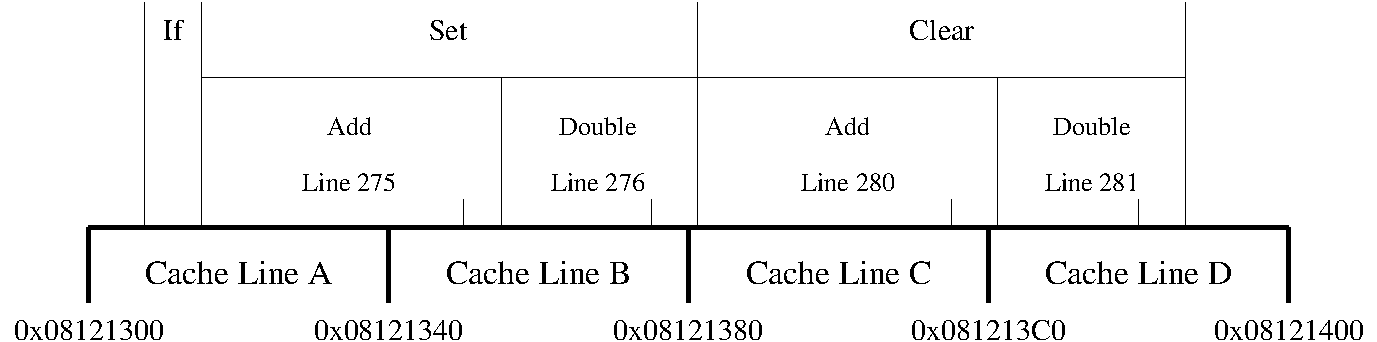
\includegraphics[width=\columnwidth]{images/memory}
\caption{Mapping from source code to memory\label{dgm:memory}}
\end{figure}


The minimum sequence of memory line accesses required for executing this code can now be constructed.
The \texttt{if} statement at line~273 is executed for each bit.  
The code of this statement is in memory line $A$, hence this memory line is accessed when processing of a bit starts.
For a set bit, the processing continues with source line~275, which maps to memory lines~$A$ and~$B$.
The actual call to the group add function occurs at address 0x08121347.
(See mark in Fig.~\ref{dgm:memory}.)
After a delay for computing the group add, execution continues in memory line~$B$ to process the return value and 
to invoke the group doubling function.
The group doubling function returns to memory line~$B$ and execution leaves the \texttt{if} body at memory line~$D$.

Hence, the sequence of memory line accesses required for a set bit is: $A$, $B$, \textit{add}, $B$, \textit{double}, $B$, $D$.
Similarly, for a clear bit, the sequence is: $A$, $C$, \textit{add}, $C$, $D$, \textit{double}, $D$.

Due to the limited temporal resolution of \fl, the attack can observe the order of memory accesses only
if they are sufficiently separated in time.
Hence, in the case of OpenSSL, the attack can only observe the order of memory accesses if they are separated by a call
to a group operation.
For example, when the bit is set, the attack cannot decide whether the access to memory line~$A$ precedes or follows the access
to memory line~$B$.
Similarly, when observed by \fl, memory accesses issued after the group double are merged with those 
issued at the start of processing the following bit.
Figure~\ref{dgm:temporal} shows the observable memory accesses when processing a set bit followed by
a clear bit.

\begin{figure}[htb]
\centering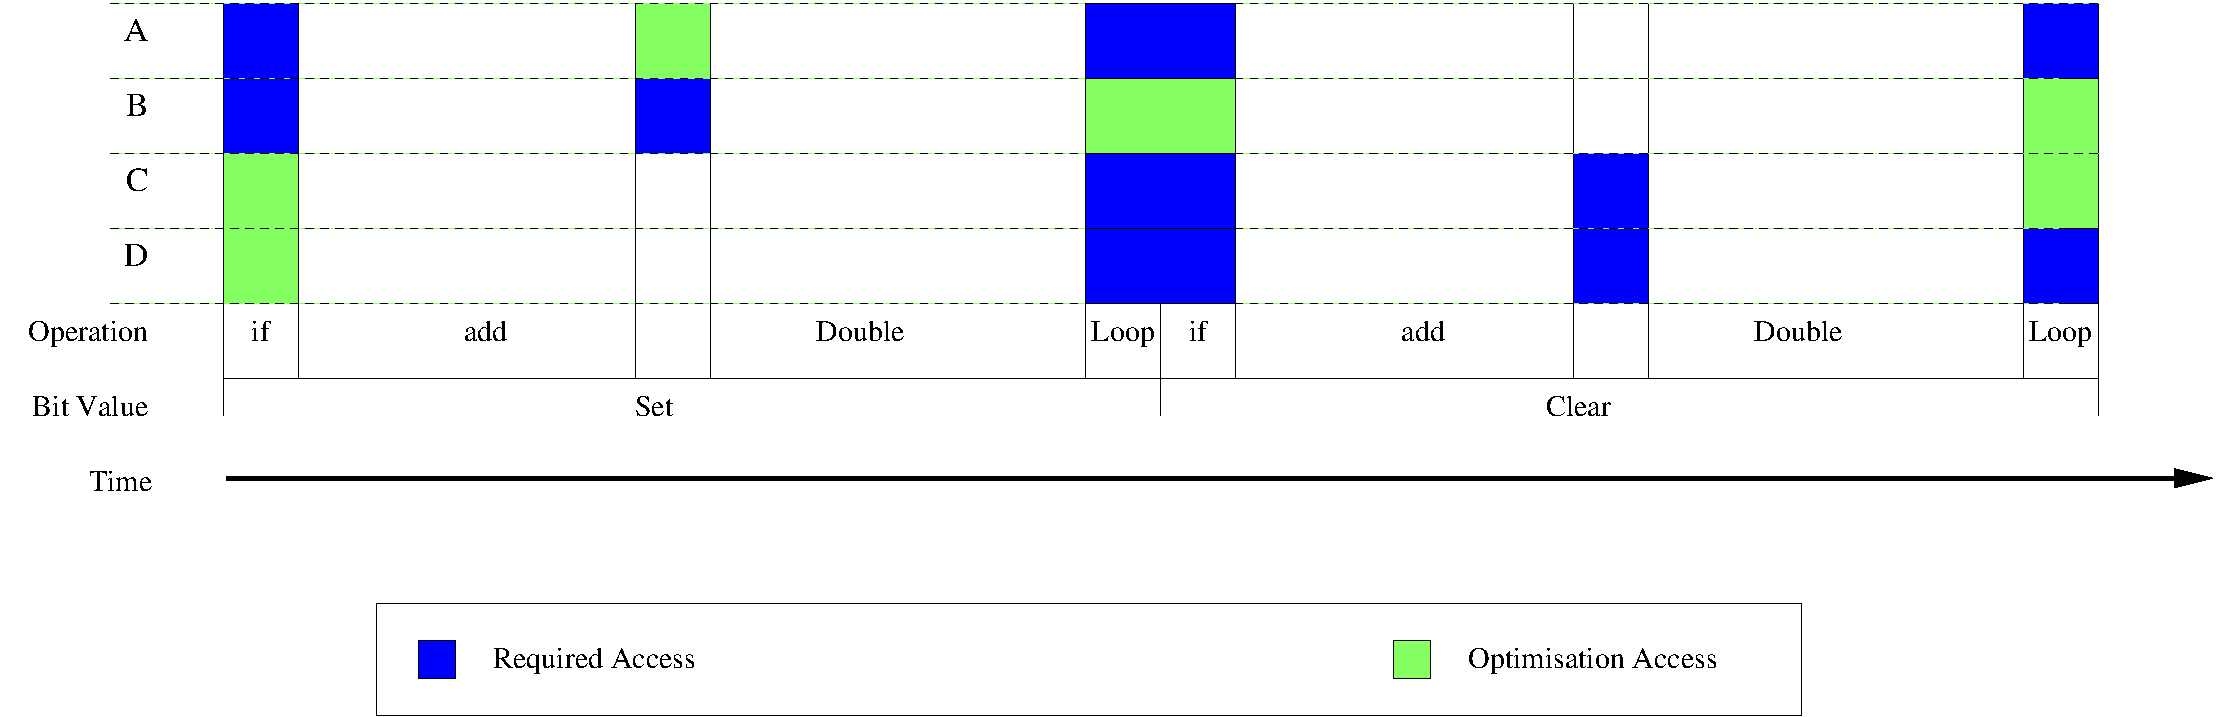
\includegraphics[width=\columnwidth]{images/temporal}
\caption{Observable memory access over time (processing a set then  a clear bit)\label{dgm:temporal}}
\end{figure}

The diagram also shows memory accesses issued by processor optimisations.
These optimisations pre-load memory lines into the cache to reduce the time the program waits for these lines.
For example, when the processor uses speculative execution~\cite{uht95disjoint}, it follows both arms of a conditional
branch before evaluating the condition.
When the condition is evaluated, the processor commits to the pre-processed computation of the correct arm,
disposing of the computation done for the other arm. 
In the case of OpenSSL this means that even before evaluating the bit, 
the processor may start processing both line~275 and line~280, triggering memory loads from memory lines~$A$, $B$ and $C$.

Another optimisation that can cause additional memory line access is spatial prefetching~\cite{intel12optimization}.
The processor pairs adjacent memory lines and tries to bring both memory lines into the cache
when there is a miss on one of the pair's lines.
For example, when there is a cache miss on memory line~$A$, the spatial prefetcher may attempt to prefetch memory line~$B$
and vice versa.

Consequently, as demonstrated in Fig.~\ref{dgm:temporal}, the memory lines accessed between computing
the group add and the group double can be used for recovering the value of the bit.
Probing any of lines~$A$ and~$B$ gives a positive indication of set bits.  
Probing either line~$C$ or~$D$ gives a positive indication of clear bits.
For our attack we probe memory lines~$B$ and~$D$.

Three limitations of the \fl attack affect its ability to capture the sequence of memory accesses.
The first is the attack temporal resolution which affects its ability to 
determine the order of accesses performed within a short time from each other.
The second limitation is the possibility of an overlap between the memory access and the probe which may result
in the attack missing the access.
The third limitation is the result of the interaction between the \fl attack and the processor
optimisation of cache use.  
In particular, the spatial prefetching optimisation implies that the attack cannot be used to probe two cache lines that form a pair,
because probing one of the lines in a pair triggers a prefetch of the other.



For OpenSSL, the attack resolution should be sufficiently high for the attack to be able to distinguish between 
memory accesses done before and after each bit and those done between the group add and group double operations of each bit.
This can be achieved by setting the time slot size to be less than the time it takes the victim to calculate the group double.
As group double calculations are faster than group add calculations, this ensures that the probed memory lines are flushed
when the victim computes the group add to be probed when the victim computes the group double.

The probability of an overlap, like the attack resolution, depends on the length of the time slot.
Longer time slots mean that the portion of time during which the spy probes is smaller and, therefore, 
the probability of an overlap is lower.

As predicted by Walter~\cite{walter04longer}, smaller keys are more resilient to the attack.
With smaller keys, group operations are shorter, forcing shorter time slots.
The shorter time slots lead to an increased probability of an overlap and with it of missing bits.

Missing memory accesses not only prevents the spy program from recovering the value of bits.
It may also result in the spy program losing the bit position in the scalar multiplication process.
To protect against this possibility, our attack also probes the first and last memory lines of the 
\texttt{gf2m\_Mdouble} function.
Probing these lines provides the spy program with additional information on the operation of the victim
and facilitates recovering the position of captured scalar bits.


The next section describes the details of our experimentation with the attack and its results.


\section{Experimental Setup and Results}\label{sec:results}

To test the attack on OpenSSL we used an HP Elite 8300 
running Fedora 18.
As the OpenSSL package shipped with Fedora does not support \myupcase{ecc},
we used our own build of OpenSSL 1.0.1e. 
To facilitate the mapping from source lines to memory addresses we built OpenSSL with debugging symbols.
In real attack settings, the attacker will need to reverse engineer~\cite{cipsero10software}
the OpenSSL library.
For the experiment we used the OpenSSL \texttt{sect1571r1} curve.
(NIST Binary-Curve B-571~\cite{fips}.)

With the selected curve, group add operations take 23,612 cycles on average.
The first group double operation takes 6,552 cycles on average, whereas further group double operations take 11,962 cycles.
Based on the discussion in Section~\ref{sec:attack}, we picked a slot length of 10,240 cycles.


\begin{figure*}[htb]
\centering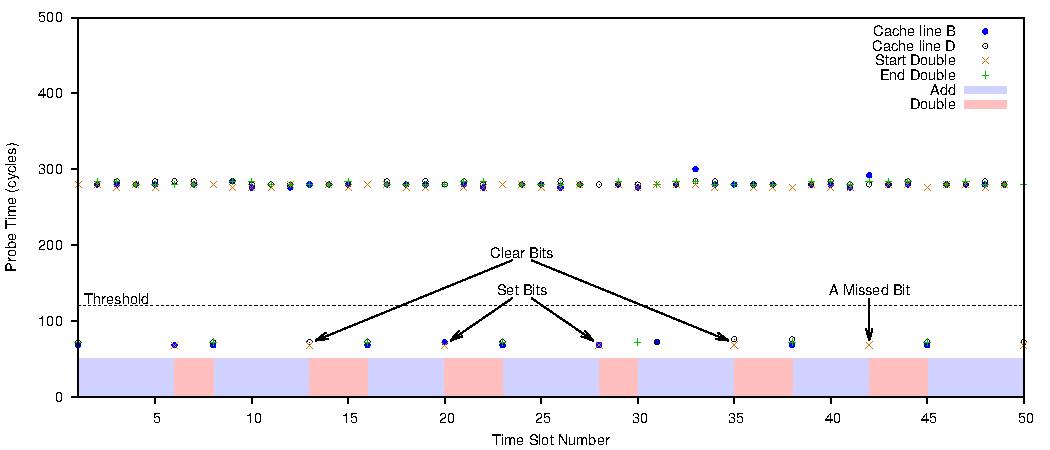
\includegraphics[width=\textwidth]{images/timing}
\caption{Probe timing during signing\label{dgm:timing}}
\end{figure*}

Figure~\ref{dgm:timing} shows the results of the probes during 50 time slots.
Probes taking less than the threshold of 120 clock cycles indicate a victim access to the probed line.
The shaded areas in the diagram indicate the computation of the group double operation, identified
by probing for group double start and end.
For clarity, we have omitted these probes from the diagram.


For example, in the first time slot, the spy program captured access to memory lines~$B$ and~$D$, as well as an access
to the last memory line of the group double.
The end of the group double is also the end of processing a bit, hence at time slot~1, the victim finished processing a bit
and started the next one.
The next captured probe is at time slot~5.
In this time slot, the victim accessed memory line~$B$ and started executing a group double.  
Access to line~$B$ between the group add and the group double operations indicates that the bit is set.
Processing the next bit starts at time slot~8 and ends in time slot~16.
The access to memory line~$D$ in time slot~13 indicates that the second bit is clear.

In the absence of access to memory lines~$B$ or~$D$ in time slot~42, the start of a group double indicates
that the spy program missed a value of a bit.
However, the fact that a bit was processed at that time slot is not missed,
demonstrating the value of probing the start of the group double operation.

\begin{figure}[htb]
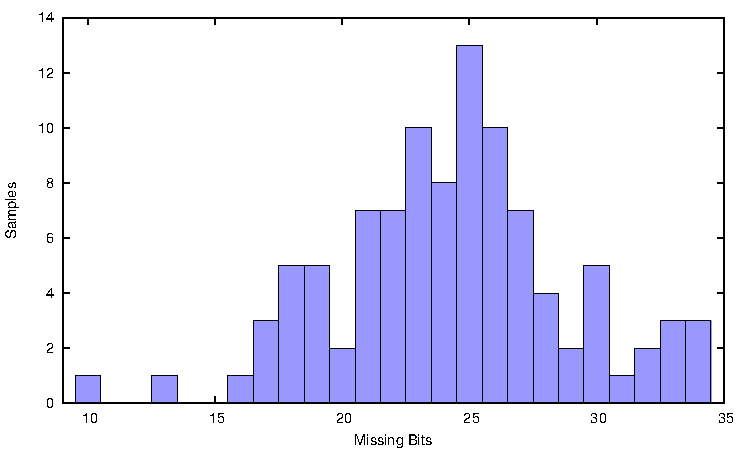
\includegraphics[width=\columnwidth]{images/missing}
\caption{Missing bits per signature\label{dgm:dist}}
\end{figure}

To measure the number of missing bits we traced the computation of~100 signatures.
On average, the attack misses only $4.26\%$ of the bits or $25.28$ bits per signature.
The distribution of number of bits missing per signature is in Fig.~\ref{dgm:dist}.
The number of missing bits ranges from 10 to 34, with the median at 25 missing bits per signature.


\begin{figure}[htb]
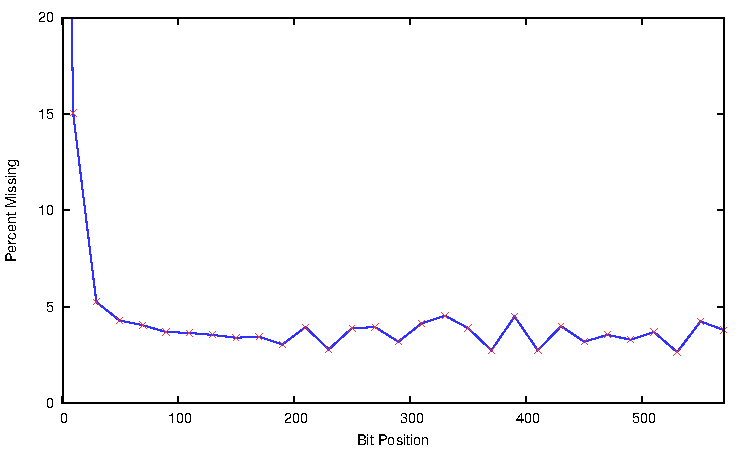
\includegraphics[width=\columnwidth]{images/positions}
\caption{Missing bits per bit position\label{dgm:missed}}
\end{figure}

As Fig.~\ref{dgm:missed} demonstrates, the distribution of missing bits position is not uniform.
The first bit (bit 0) is always missed.
This is mostly the result of the short time it takes OpenSSL to compute the group double operation for the first bit.
Even ignoring the first bit, it is evident that missing bits tend to cluster towards the most significant bits of the
scalar.
Around 15\% of the bits in positions~1 to~20 are missed, compared with 3.6\% of the bits from position 50 onward,
where the distribution of missing bits is approximately uniform.





\section{Discussion}\label{sec:discussion}

\subsubsection*{Full Recovery of the Nonce}\label{sub:full_nonce}
Given the high proportion of nonce bits recovered by the \fl attack, using the LLL based techniques~\cite{Howgrave-GrahamS01,nguyen03insecurity} described in Sect.~\ref{sec:related} seems computationally excessive. 
With a worst case of 34 bits missing, the baby step giant step algorithm~\cite{shanks71class} would require less then 10 Megabytes of memory and less than one second of computation to complete the nonce.

%There are a number of attacks on \myupcase{ecc} protocols which recover the secret key using a small proportion of the leaked nonce. In this attack, the proportion of the nonce recovered by the \fl attack is significantly higher; using one of the existing attacks would be unnecessarily (computationally) excessive. %Attacks using lattice techniques to solve the related hidden number problem, for example, ... In experiments a basic BSGS implementation sufficed... 

\subsubsection*{Implications}

As the \myupcase{ecdlp} is not targeted by this attack, the signature protocol is made no more vulnerable by our results. 
This attack targets the scalar multiplication implementation of OpenSSL and is therefore particular to implementations using this and similar implementations of the Montgomery ladder. The vulnerability introduced by this implementation is due to the bits of the secret nonce determining which conditional branch is taken. 
%We monitor the branching to determine the value of the bits. This is clearly an attack which needs to be combated by both software and hardware cooperatively: 
Our spy program is able to determine how the algorithm executes by having access to the victim's memory and used this knowledge to reconstruct values used by the software.


As demonstrated in this paper, the \fl attack  has a higher resolution and  better accuracy then previously known attacks.
\fl applies across multiple cryptographic schemes and we show that it applies
to implementation hitherto not considered vulnerable to side-channel attacks.
It, therefore, presents new threats to confidentiality of data.

This threat is not limited to cryptographic software.
The attack can be applied to other software and may be able to extract sensitive information from other software,
including keystroke timing information~\cite{song01timing,ristenpart09hey}, statistical data on network traffic and disk use
and business logic.

\subsubsection*{Mitigation}

%To successfully extract sensitive data using the technique we describe, the victim program must have a branch which depends on sensitive data, 
%the code of the victim  must be shared with the spy program and the spy program should be allowed to use the \texttt{clflush} command on the shared code.
%Breaking any of these three dependency mitigates the attack.

Preventing data flow from secrets to branch conditions is one way for mitigating the attack.
The Networking and Cryptography library (NaCl), implemented by Bernstein, Lange and Schwabe~\cite{dan-tan-peter}, 
provides an implementation of the Montgomery ladder that is not vulnerable to our attack.
Instead of using branches, NaCl uses arithmetic operations to select the arguments and targets of the group operation.
Consequently, NaCl's use of the cache is independent of the values of the bits in the nonce.
Fixing OpenSSL by using methods similar to those used in NaCl will provide protection against the attack.

While fixing OpenSSL would prevent the attack we describe, it is not a panacea for the \fl attack.
As discussed above, the attack is generic and can apply to other software.
%It is hard to expect every software that manipulates sensitive data to be re-written to avoid any data flow from the sensitive data to branch conditions. Consequently, a hardware fix to prevent the unfettered use of the \texttt{clflush} instruction is required.
It would be advisable for implementors of cryptographic software to avoid using secret information to determine which operations 
or values are accessed when the memory locations can be distinguished by an eavesdropper. 


The \fl technique exploits the lack of restrictions
on the ability to flush specific memory lines from the cache,
which enables processes
to interact using read-only pages.
This is a security weakness of the
IA32 and the X86-64 architectures.
Addressing this weakness requires a hardware fix.
A possible fix is 
to restrict  the ability to flush memory to
memory pages to which the process has write access and to
memory pages to which the system allows such access.
This access control could be implemented by adding memory
types that restrict flush access to the PAT (Page Attribute
Table)~\cite[chap. 11]{intel13architecture:3a}

%In the Networking and Cryptography library (NaCl), implemented by Daniel J. Bernstein, Tanja Lange and Peter Schwabe, there is no data flow from secrets to branch conditions, precisely the vulnerability of the OpenSSL implementation targeted by this attack. Analysis of the core security features of NaCl is given in Bernstein et al.~\cite{dan-tan-peter}. The attack presented in this article relies on distinguishing bits of the nonce by observing the branching in traditional Montgomery ladder implementation. As the NaCl library avoids branching dependent on secret parameters this attack is not applicable to NaCl's \url{crypto_sign} API. (NaCl is in the public domain and has been made available by the authors of Bernstein et al.~\cite{dan-tan-peter} at \url{http://nacl.cr.yp.to}.)


\section{Conclusions and future work}
The results of this work imply that the OpenSSL Montgomery ladder implementation should be avoided in 
all implementations of elliptic curve protocols when a scalar multiplication step involves a secret parameter. 
This attack is applicable when the malicious party has access to the memory of the targeted device, 
a completely reasonable assumption, possible when using a multi-user operating system, a virtual machine or a computer victim to malware. 

The results of this work also support the theory of Walter~\cite{walter04longer} that smaller keys are more resilient to side-channel analysis.
In this attack a higher proportion of the nonce can be obtained for larger key sizes. 
This implies that as we, naturally, transition to larger parameters in response to increasing computing capabilities, 
prevention of side-channel attacks should be incorporated into the implementation design, 
as is the methodology adopted by the authors of the NaCl cryptographic library \cite{dan-tan-peter}. 

Further work in this line of research is to apply the \fl attack outside the realm of scalar multiplication.
A possible use is for implementing the Vaudenay padding oracle attack~\cite{alfardan12plaintext,vaudenay02security}.
It would also be interesting to test the extent to which the attack can be applied to non-cryptographic software.
The nature of the threat the attack presents to business logic and to customer privacy should be evaluated.




%There are a number of future directions for this research, including the development of the use of Gray codes in improving the BSGS method to extend the efficiency of obtaining the full scalar from a partially obtained secret. It would also be usedful to understand what proportion of the nonce should be obtained for the BSGS method to become more practical than the LLL method. 

\begin{acknowledgements}
The authors wish to thank Dr Katrina Falkner for the advice and support.

This research was performed under contract to the Defence
Science and Technology Organisation (DSTO) Maritime Division,
Australia.
\end{acknowledgements}

%\starpar{Bitcoin uses ECDSA}~\cite{nakamoto--bitcoin}

\bibliographystyle{splncs}
\bibliography{Euro2014}

\end{document}

